\chapter{Cómputo bayesiano}

De acuerdo con \textcite{Ross10}, los resultados más importantes y más conocidos de la teoría de probabilidad son los llamados teoremas límite, en particular aquellos conocidos como \textit{leyes de los grandes números}. La idea general podemos tomarla de Jakob Bernoulli, el primero en presentar un teorema de este tipo, y estriba en que todos los hombres saben ``por algún instinto de la naturaleza \textit{per se} y sin ninguna instrucción previa, que entre más observaciones hay, menor es el peligro de alejarse del blanco" \parencite{Pulskamp09}. Es decir, si tenemos suficientes realizaciones de un experimento, podemos estimar con mucha precisión aquello que buscamos.\\

Hoy tenemos--- después de varios avances históricos que pueden consultarse en \textcite{Seneta13}--- las siguientes dos leyes generales de los grandes números, cuyas pruebas bajo algunos supuestos adicionales pueden consultarse en \textcite{Ross10}:

\begin{teo} \label{teo:LGN}
\textbf{Leyes de los grandes números.}
Sean $X_1,\,X_2,\dots$ una secuencia de variables aleatorias independientes e idénticamente distribuidas, cada una con media finita $E[X_i]=\mu$, y $\bar{X}_N=\sum\limits_{i=1}^N\dfrac{X_i}{N}$, las respectivas medias empíricas. Entonces se cumplen las siguientes dos leyes.
\begin{itemize}
\item \textbf{Ley débil}
\begin{equation*}
\lim_{N \to \infty} P\left( |\bar{X}_N-\mu| \geq \epsilon \right)  = 0 \qquad \forall \, \epsilon > 0
\end{equation*}
\item \textbf{Ley fuerte}
\begin{equation*}
P\left(\lim_{N \to \infty} \bar{X}_M = \mu \right)  = 1 
\end{equation*}
\end{itemize}
\end{teo}

Ambas leyes nos dicen que, conforme el tamaño de una muestra aleatoria aumenta, los promedios empíricos convergen a los promedios teóricos. Una manera común de ejemplificar este fenómeno es mediante el lanzamiento sucesivo de monedas. En este caso los volados \textit{simulan} observaciones de una variable aleatoria de ensayos Bernoulli y, al tener una muestra suficientemente grande, se comienza a apreciar la convergencia hacia la probabilidad de éxito.\\ 

Gracias al avance tecnológico, hoy ya no tenemos necesariamente que lanzar volados físicamente sino que los simulamos desde una computadora, a partir de la generación de números pseudoaleatorios, diseñados de manera tal que satisfagan todas las propiedades básicas de números auténticamente aleatorios \parencite{Ross13}. Podemos pedirle a la computadora que simule una gran cantidad de volados y registre la proporción empírica acumulada de los que cayeron águila. Conforme más aumenta el número de volados, más nos acercamos a 0.5, la proporción teórica. Esto se puede repetir para otras series de volados y el comportamiento es el mismo, como puede apreciarse en la \textbf{Figura \ref{fig:LGN}}. \\

\begin{figure}[h]
	\centering
	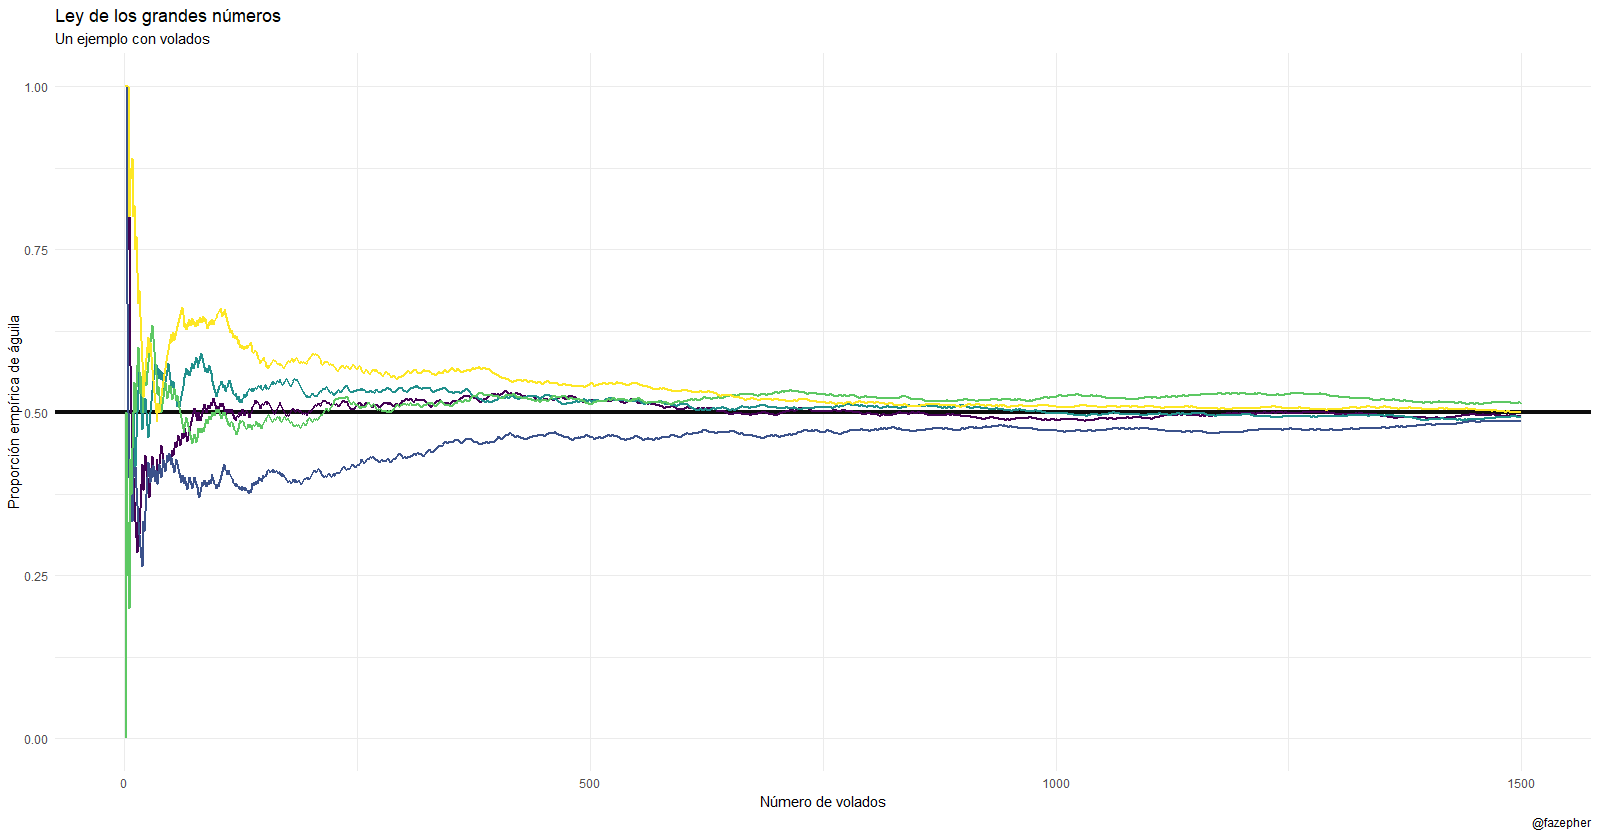
\includegraphics[scale=0.25]{Figs/LGN}
	\caption{Ilustración de las leyes de los grandes números mediante volados simulados por computadora. Conforme el número de volados aumenta, la proporción empírica converge a la proporción teórica. Esto pasa para cada serie de volados. Fuente: elaboración propia.}
	\label{fig:LGN}	
\end{figure}

Es cierto que esta práctica de aprender de un sistema, simulando con muestreo aleatorio no surge con las computadoras \parencite{Owen13}. Ya desde 1812 Laplace había sugerido la posibilidad de estimar empíricamente el valor de $\pi$ mediante el llamado problema de la aguja de Buffon \parencite{Ragheb13}. Sin embargo, como el ejemplo de los volados muestra, sí han sido las computadoras las que han potenciado la utilidad de los métodos de simulación. ¿Cuánto hubiéramos tardado en lanzar los 7,500 volados que la computadora simuló al instante? Más aún, esta capacidad computacional consolidó la utilidad de la estadística bayesiana. ¡Y pensar que todo empezó con una guerra y un juego de solitario!, como explico a continuación.

\section{Monte Carlo} 

La simulación por computadora ha permitido el desarrollo de la estadística bayesiana, particularmente desde la década de los 90 del siglo pasado \parencite{RobertCasella11}. Sin embargo, la semilla de este desarrollo ya había sido plantada medio siglo antes desde el terreno de la física, desafortunadamente a causa de la Segunda Guerra Mundial, por los científicos del laboratorio de Los Alamos, encargados del proyecto Manhattan y el desarrollo de más armas de fisión nuclear.\\

Uno de esos científicos fue un matemático polaco-estadounidense llamado Stanislaw Ulam. En 1946, aburrido convaleciendo por una enfermedad, comenzó a preguntarse sobre la probabilidad de ganar en un juego de solitario. Después de mucho batallar con los cálculos de combinatoria se planteó si no sería más práctico estimarla simulando muchas partidas en una de las primeras computadoras electrónicas. Y ahí surgió el eureka: ¿por qué no hacer lo mismo para los problemas de física nuclear en los que estaban trabajando en Los Alamos? \parencite{Eckhardt87}. Al igual que las partidas de solitario, podrían simular muchas realizaciones de los procesos físicos bajo estudio y estimar los resultados más probables.\\ 

Stan compartió su idea con John von Neumann quien, sorprendido y emocionado con la idea, le envió una carta a Richard Richtmayer--- el líder del equipo en Los Alamos--- con todos los cálculos necesarios para llevar a cabo el proyecto \parencite{vonNeumann47}. El método fue rápidamente adoptado por todos en Los Alamos, tanto que otro físico, Nicholas Metropolis, sugirió llamarlo \textit{Monte Carlo}, bromeando sobre un tío apostador de Stan, que vivía pidiendo prestado dinero porque ``simplemente tenía que ir a Monte Carlo" \parencite{Metropolis87}. Después de un arduo trabajo, el método pareció funcionar--- gracias en buena medida al trabajo de programación de Klara von Neumann \parencite{Haigh14}--- y el propio Metropolis publicó, junto con Stan, un primer paper presentándolo a grandes rasgos \parencite{MetropolisUlam49}.\\

De manera concreta, el método es la conjunción de la simulación con la ley de los grandes números. Las cantidades que requerían calcular eran valores esperados de la siguiente forma: 
\begin{equation}
\label{eq:IntegralMC}
h^\star = \mathbb{E}[h(X)]=\int\limits_\mathcal{X} h(x)f(x)dx ,
\end{equation} 
donde $h$ es una función de interés y $f(x)$ es la distribución de probabilidad sobre las \textit{configuraciones} en las que podía encontrarse el sistema físico. Estas integrales típicamente no pueden calcularse ni analíticamente ni por métodos numéricos tradicionales. Sin embargo, si se tiene una muestra aleatoria de valores de $X$ provenientes de su distribución $f$, se puede aproximar $\bar{h}$ con el promedio empírico, que en este contexto se conoce como \textit{estimador de Monte Carlo}: 
\begin{equation*}
h^\star \approx \hat{h} = \sum\limits_{i=1}^N \dfrac{h(x_i)}{N}
\end{equation*}

El problema para los científicos en Los Alamos se convirtió entonces en encontrar algoritmos eficientes para obtener una muestra aleatoria de variables provenientes de diferentes distribuciones $f$.\\ 

Este problema es exactamente el mismo que se tiene en la aplicación de la estadística bayesiana. En efecto, la forma de la \textbf{Ecuación \ref{eq:IntegralMC}} permite llevar a cabo una gran variedad de \textit{resúmenes inferenciales} \parencite{GP97}. La posibilidad de realizar la correspondiente \textit{integración por Monte Carlo} hace que, en la práctica, exista una dualidad entre una distribución o densidad y una muestra proveniente de ella \parencite{SmithGelfand92}. La única receta de la inferencia bayesiana--- ver la página \pageref{receta_bayesiana}---, en la práctica se convierte en obtener una muestra aleatoria de la distribución posterior lo suficientemente grande para, con ella, estimar por Monte Carlo los resúmenes inferenciales requeridos.\\

Hay varios métodos de simulación de variables aleatorias que permiten obtener muestras aleatorias independientes y calcular un estimador de Monte Carlo. Entre los más mencionados podemos encontrar el método de inversión, el de aceptación y rechazo o el muestreo por importancia. Sin embargo, los físicos de Los Alamos pronto se dieron cuenta que podrían ser más eficientes si, en lugar de buscar realizar simulaciones independientes, hacían simulaciones secuenciales que dependieran entre sí. 

\section{MCMC}

La forma de realizar simulaciones correlacionadas que logren simular de manera más eficiente que los métodos tradicionales de aceptación y rechazo o muestreo por importancia es utilizar \textit{cadenas de Markov}.

\dfn{\textbf{Cadena de Markov}\\
\label{def:Cadena_Markov}
Una \textit{cadena de Markov} $\left\lbrace X_{(n)}, \, n = 0, 1, 2,\dots \right\rbrace$ es una secuencia de variables aleatorias tales que satisfacen la siguiente \textit{propiedad de Markov} para toda $n$
\begin{equation*}
X_{(n+1)}| X_{(n)}, \dots, X_{(0)} \sim X_{(n+1)}| X_{(n)} \sim p(x_{(n)},\tilde{x}_{(n+1)})
\end{equation*}
}

Si llamamos \textit{estados} a los eventos que suceden en la cadena en cada punto en el tiempo, podemos decir que la distribución condicional del estado futuro de una cadena de Markov dada toda su historia depende exclusivamente del estado presente y no de los estados anteriores. Esta distribución condicional se llama \textit{kernel de transición}, mismo que normalmente es independiente del índice $n$ y depende exclusivamente del estado actual y el estado futuro. Esta propiedad se llama \textit{homogeneidad} en el tiempo y permite simplificar la notación a $p(x,\tilde{x})$.\\ 

La teoría de cadenas de Markov determina las condiciones bajo las cuales existen teoremas límites al estilo de las leyes de los grandes números y que en este contexto se conocen como \textit{ergódicos}. Esta teoría escapa los objetivos particulares de la tesis pero, si es de interés para el lector, algunas referencias útiles son {\color{Red} Citar libros de estocásticos}. Baste decir por ahora que, bajo ciertas condiciones, sabemos que la distribución de $X_{(n)}$ converge a una distribución límite conforme $n$ tiende a infinito. Más aún, los \textit{promedios ergódicos}--- es decir los promedios acumulados de la cadena--- también convergen al valor esperado de la distribución límite.\\ 

Esto da lugar a los métodos de \textit{Markov Chain Monte Carlo} o MCMC en los que el objetivo es construir una cadena de Markov que satisfaga las condiciones del teorema ergódico y cuya distribución límite sea la distribución de la cuál se quiere simular. Así, después de $N$ transiciones de la cadena, la distribución de los valores simulados sería aproximadamente la distribución objetivo y se podría estimar la cantidad de interés $h^\star$ mediante el estimador de MCMC: 

\begin{equation*}
h^\star \approx \hat{h} = \sum\limits_{i=n}^N \dfrac{h(x_{(n)})}{N}
\end{equation*}

\subsection{Metropolis-Hastings}

 El primero de estos métodos MCMC fue propuesto por las parejas de esposos Arianna y Marshall Rosenbluth y Augusta y Edward Teller junto con el propio Nicholas Metropolis en el \textit{Journal of Chemical Physics} \parencite{Metropolis53}. Se conoce como el algoritmo de Metropolis, aunque hay quienes creen que en realidad el trabajo más fuerte lo hicieron el resto de los autores por lo que debería llamarse el algoritmo de Rosenbluth-Teller {\color{Red} citar Gubernatis}. Casi 20 años después de esta propuesta desde el terreno de la física, el estadístico canadiense Wilfred Keith Hastings lo generalizó {\color{Red} citar Hastings}, por lo que podemos hablar de algoritmos de Metropolis-Hastings o MH.\\
 
Las cadenas de Markov para MH requieren ser homogéneas en el tiempo y que sea posible llegar a cualquier estado en un número finito de transiciones, algo que se conoce como \textit{irreducibilidad}. Si además de ser una cadena irreducible, el kernel de transición satisface la siguiente \textit{ecuación de balance detallado} para alguna distribución $f$, se dice que es reversible y podemos aplicar el teorema ergódico.
\begin{equation}
\label{eq:Balance_Detallado}
f(x)p(x,\tilde{x})=f(\tilde{x})p(\tilde{x},x)
\end{equation}

El algoritmo de Metropolis-Hastings busca construir cadenas de Markov homogéneas, irreducibles y reversibles que tengan como distribución límite a la distribución objetivo. ¿Cómo hacerlo? Para ello analicemos lo que la reversibilidad implica de manera intuitiva.\\

Siguiendo la argumentación de {\color{Red} Citar Chib y Greenberg}, la \textbf{Ecuación \ref{eq:Balance_Detallado}} refleja que hay un balance entre las probabilidades de la cadena de estar en diferentes estados, de ahí el nombre. Supongamos que no se cumpliera la reversibilidad para algún kernel $q(x,\tilde{x})$. Entonces, sin pérdida de generalidad, para algunos estados pasaría que:
\begin{equation}
\label{eq:Inbalance_Detallado}
f(x)q(x,\tilde{x})>f(\tilde{x})q(\tilde{x},x) \quad \Rightarrow \quad \dfrac{f(x)}{f(\tilde{x})}>\dfrac{q(\tilde{x},x)}{q(x,\tilde{x})}
\end{equation}

De manera un poco informal, tenemos que el miembro izquierdo de la segunda desigualdad refleja las probabilidades relativas ``necesarias'' entre estar en el estado $x$ y el estado $\tilde{x}$. El miembro derecho, por su parte, indica las probabilidades relativas de transitar a dichos estados bajo el kernel de transición de la cadena. La desigualdad indica que la cadena estaría transitando de $x$ a $\tilde{x}$ más de lo necesario y, equivalentemente, transitando de $\tilde{x}$ a $x$ menos de lo necesario.\\ 

Para conseguir el balance necesario para aplicar el teorema ergódico, necesitamos hacer una \textit{corrección de Metropolis} al kernel de transición, reduciendo el número relativo de veces que la cadena transite de $x$ a $\tilde{x}$ y aumentando el número relativo de transiciones de $\tilde{x}$ a $x$. La forma de hacer la corrección es comenzar con un kernel de transición $q(x,\tilde{x})$ que \textit{proponga} un estado y agregar una \textit{probabilidad de aceptación} $\alpha(x,\tilde{x})$ de que el estado propuesto se acepte. Si la propuesta se rechaza, la cadena permanece en el mismo estado, reduciendo a la vez el número de transiciones hacia estados sobremuestreados y aumentando el número relativo de veces que estamos en el estado originalmente submuestreado. Estos dos pasos constituyen un nuevo kernel de transición de Metropolis-Hastings de la siguiente forma: 
\begin{align*}
p_{MH}(x,\tilde{x}) &= q(x,\tilde{x})\alpha(x,\tilde{x}) \quad x \neq \tilde{x} \\
p_{MH}(x,x) &= 1 - \int\limits_\mathcal{X} p_{MH}(x,\tilde{x})d\tilde{x}
\end{align*}

Queremos que el kernel $p_{MH}$ satisfaga la \textbf{Ecuación \ref{eq:Balance_Detallado}}, entonces:
\begin{equation*}
f(x)p_{MH}(x,\tilde{x})=f(\tilde{x})p_{MH}(\tilde{x},x) \quad \Leftrightarrow \quad f(x)q(x,\tilde{x})\alpha(x,\tilde{x})=f(\tilde{x})q(\tilde{x},x)\alpha(\tilde{x},x) 
\end{equation*}

Las transiciones de $\tilde{x}$ a $x$ se dan demasiado poco, de acuerdo a nuestra desigualdad supuesta en \textbf{\ref{eq:Inbalance_Detallado}}. Por lo que deberíamos siempre aceptar este tipo de transiciones a fin de corregir el submuestreo. Tomemos entonces $\alpha(\tilde{x},x) = 1$ y observemos que $\alpha(x,\tilde{x})$ queda determinada de tal forma que logremos el balance necesario: 
\begin{equation*}
\alpha(x,\tilde{x})=\dfrac{f(\tilde{x})q(\tilde{x},x)}{f(x)q(x,\tilde{x})}
\end{equation*}

Si la desigualdad \textbf{\ref{eq:Inbalance_Detallado}} fuera en el sentido contrario, i.e. $f(\tilde{x})q(\tilde{x},x)>f(x)q(x,\tilde{x})$, los roles de las probabilidades de aceptación se invertirían, por lo que de manera general tenemos que 
\begin{equation}
\label{eq:Proba_Aceptar_MH}
\alpha(x,\tilde{x})=min\left[\dfrac{f(\tilde{x})q(\tilde{x},x)}{f(x)q(x,\tilde{x})},1\right]
\end{equation}
